\chapter{การวิเคราะห์ความซับซ้อน (Complexity Analysis)}

การเขียนโปรแกรมแก้ปัญหานั้น นอกจากคำนึงถึงความถูกต้องในการแก้ปัญหาแล้ว สิ่งที่ควรต้องคำนึงถึงหลักๆ ได้แก่ เวลาที่ใช้ในการทำงาน (Time complexity) และหน่วยความจำที่ใช้ในการทำงาน (Space complexity)

การวิเคราะห์ความซับซ้อนของโปรแกรม คือกระบวนการในการตัดสินว่าโปรแกรมไหนมีประสิทธิภาพมากกว่ากัน โดยตัดปัจจัยอื่นที่ไม่เกี่ยวข้องทิ้งไป เช่น ความเร็วในการทำงานของคอมพิวเตอร์แต่ละเครื่องที่แตกต่างกัน เป็นต้น

\section{สัญกรณ์เชิงเส้นกำกับ (Asymptotic Notation)}

สัญกรณ์เชิงเส้นกำกับ เป็นสัญกรณ์เพื่อบอกการทำงานของโปรแกรมนั้นๆ ซึ่งประกอบไปด้วย

\begin{example}
ฟั่งก์ชั่นค้นหาตำแหน่งของตัวเลขที่ต้องการภายในอาเรย์ที่ชื่อว่า \texttt{numberList}
\begin{lstlisting}
int findSpecificNumberPosition(int n, int targetNumber){
	for (int i = 0; i < n; i++){
		if (numberList[i] == targetNumber){
			return i;
		}
	}
	return -1;
}
\end{lstlisting}
การทำงานของฟังก์ชั่นนี้คือตรวจสอบตัวเลขที่ต้องการไปทีละตำแหน่ง โดยเริ่มจากตำแหน่งที่ 1 ไปยังตำแหน่งที่ \texttt{n-1} หากพบ จะคืนค่าตำแหน่งนั้น หากไม่พบจะคืนค่า -1 ออกมา
\end{example}

\subsection{สัญกรณ์โอใหญ่ (Big-O Notation)}

Big-O ถูกใช้เพื่อแสดงเวลาการทำงานที่\textbf{แย่ที่สุด}ของโปรแกรม เราสามารถคำนวนได้จากการนับจำนวนครั้งการทำงานในกรณีที่แย่ที่สุด สัญกรณ์นี้มักจะถูกใช้ในการวิเคราะห์โปรแกรมเพื่อวางแผนเผื่อกรณีที่แย่ที่สุดไว้เสมอ

จากตัวอย่าง 4.1.1 ในกรณีที่แย่ที่สุด คือต้องทำการตรวจสอบทั้งหมด \texttt{n} ครั้ง (ตรวจสอบทั้งอาเรย์) จึงจะเจอเลขที่ต้องการ แสดงว่าฟังก์ชั่นนี้มี Big-O คือ $O(n)$

\subsection{สัญกรณ์โอเมกาใหญ่ (Big-$\Omega$ Notation)}

Big-$\Omega$ ถูกใช้เพื่อแสดงเวลาการทำงานที่\textbf{ดีที่สุด}ของโปรแกรม เราสามารถคำนวนได้จากการนับจำนวนครั้งการทำงานในกรณีที่ดีที่สุด

จากตัวอย่าง 4.1.1 ในกรณีที่ดีที่สุด คือทำการตรวจสอบเพียงครั้งเดียว (ตำแหน่งแรกของอาเรย์) แล้วเจอเลขที่ต้องการทันที แสดงว่าฟังก์ชั่นนี้มี Big-$\Omega$ คือ $\Omega(1)$

\subsection{สัญกรณ์ทีตาใหญ่ (Big-$\Theta$ Notation)}

Big-$\Theta$ ถูกใช้เพื่อแสดงเวลาการทำงานที่เท่ากันของโปรแกรมทั้งในกรณีที่ดีที่สุดและกรณีที่แย่ที่สุด เราสามารถคำนวนได้จากการนับจำนวนครั้งการทำงานในกรณีที่ดีที่สุด และนับจำนวนครั้งการทำงานในกรณีที่แย่ที่สุด หากเท่ากัน จึงจะได้ Big-$\Theta$ ออกมา หากไม่เท่ากัน หมายความว่าโปรแกรมนั้นไม่มี Big-$\Theta$

จากตัวอย่าง 4.1.1 
\begin{itemize}
\item ในกรณีที่ดีที่สุด คือทำการตรวจสอบเพียงครั้งเดียว (ตำแหน่งแรกของอาเรย์) แล้วเจอเลขที่ต้องการทันที แสดงว่าฟังก์ชั่นนี้มี Big-$\Omega$ คือ $\Omega(1)$
\item ในกรณีที่แย่ที่สุด คือต้องทำการตรวจสอบทั้งหมด \texttt{n} ครั้ง (ตรวจสอบทั้งอาเรย์) จึงจะเจอเลขที่ต้องการ แสดงว่าฟังก์ชั่นนี้มี Big-O คือ $O(n)$
\end{itemize}
จึงสรุปได้ว่าฟังก์ชั่นตัวอย่าง 4.1.1 ไม่มี Big-$\Theta$

\begin{example}
ฟังก์ชั่นแสดงผลตัวเลขทั้งหมดในอาเรย์ \texttt{numberList}
\begin{lstlisting}
void printAllNumber(int n){
	for (int i = 0; i < n; i++){
		cout << numberList[i] << endl;
	}
}
\end{lstlisting}
การทำงานของฟังก์ชั่นนี้จะแสดงผลตัวเลข เริ่มจากตำแหน่งที่ 1 ไปยังตำแหน่งที่ \texttt{n-1} รวมทั้งสิ้น \texttt{n} จำนวน
\end{example}

จากตัวอย่าง 4.1.2 ไม่ว่าจะกรณีที่ดีที่สุดหรือแย่ที่สุด ฟังก์ชั่นนี้ต้องแสดงผลตัวเลขทั้ง \texttt{n} จำนวนออกมา จึงได้ว่ามี $O(n)$, $\Omega(n)$, และ $\Theta(n)$

\newpage

\begin{figure}[h!]
    \centering
    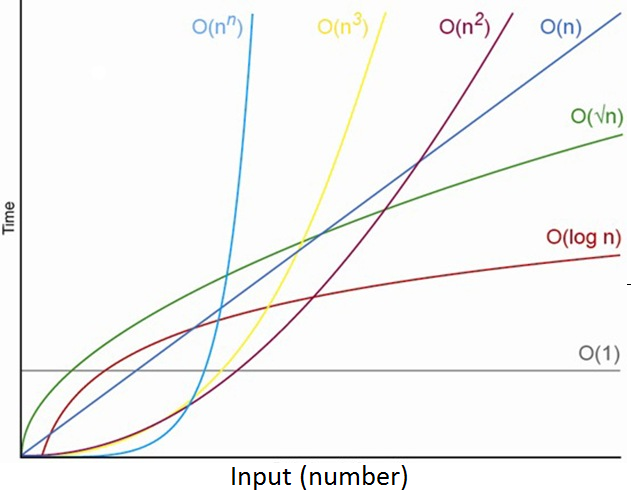
\includegraphics[width=13cm]{images/time_complex_graph}
    \caption{ตัวอย่างกราฟความสัมพันธ์ระหว่างข้อมูลนำเข้าและเวลาการทำงาน}
    \label{fig:time-complex-graph}
\end{figure}

\begin{figure}[h!]
    \centering
    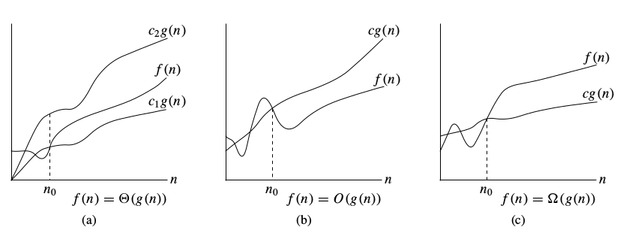
\includegraphics[width=13cm]{images/graph_3_cases}
    \caption{กราฟแสดงการวิเคราะห์สัญกรณ์เชิงเส้นกำกับทั้ง 3 ชนิด}
    \label{fig:graph-3-cases}
\end{figure}

การวิเคราะห์เวลาการทำงาน สามารถละค่าคงตัวได้ เช่น หากมีฟังก์ชั่นหนึ่งที่ใช้เวลาการทำงานน้อยกว่า $3n^2$ จะสามารถกล่าวได้ว่า ฟังก์ชั่นนี้มี $O(n^2)$

ในรูป 4.2 (a) จะเห็นได้ว่า เวลาที่ฟังก์ชั่น $f(n)$ ใช้ในการทำงานมีค่าอยู่ระหว่าง $c_1g(n)$ และ $c_2g(n)$ โดยที่ $c_1$ และ $c_2$ เป็นค่าคงตัว จึงสามารถสรุปได้ว่า $f(n)=\Theta(g(n))$

ในรูป 4.2 (b) จะเห็นได้ว่า เวลาที่ฟังก์ชั่น $f(n)$ ใช้ในการทำงานมีน้อยกว่า $cg(n)$โดยที่ $c$ เป็นค่าคงตัว จึงสามารถสรุปได้ว่า $f(n)=O(g(n))$

ในรูป 4.2 (c) จะเห็นได้ว่า เวลาที่ฟังก์ชั่น $f(n)$ ใช้ในการทำงานมีมากกว่า $cg(n)$โดยที่ $c$ เป็นค่าคงตัว จึงสามารถสรุปได้ว่า $f(n)=\Omega(g(n))$

\section{การวิเคราะห์การเวียนบังเกิด (Recurrence Analysis)}

การวิเคราะห์ฟังก์ชั่นเวียนบังเกิดอาจใช้การนับโดยตรงได้ยาก เนื่องจากการทำงานที่เรียกตัวเองซำ้ไปเรื่อยๆ จึงมีแนวทางการวิเคราะห์อยู่ ดังนี้

\subsection{Recursion Tree}

Recursion tree เป็นเครื่องมือที่เป็นประโยชน์ในการจำลองสิ่งที่เกิดขึ้นเมื่อมีการเวียนบังเกิด โดยแต่ละปมของต้นไม้จะแทนด้วยจำนวนคำสั่งที่ถูกเรียกใช้ในการเวียนบังเกิดแต่ละครั้ง

\begin{example}
$T(n)=2T(\frac{n}{2}) + n^2$

\begin{figure}[h!]
    \centering
    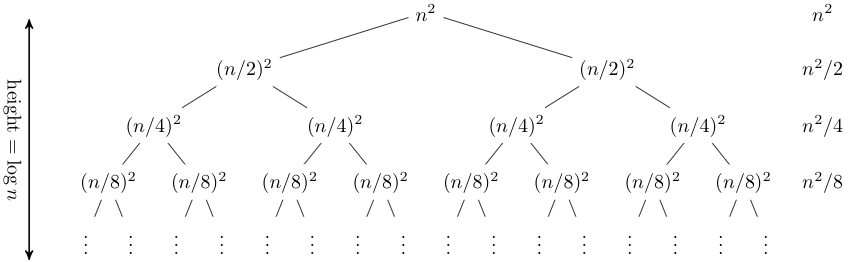
\includegraphics[width=13cm]{images/tree-2-2-2}
    \caption{Recursion tree ของการเวียนบังเกิด $T(n)=2T(\frac{n}{2}) + n^2$ }
    \label{fig:tree-2-2-2}
\end{figure}
จากรูป 4.3 จะเห็นได้ว่าชั้นบนสุดมีผลรวมของจำนวนคำสั่งมากที่สุด คือ $n^2$ ในขณะที่ชั้นอื่นๆ มีจำนวนคำสั่งรวมน้อยกว่า $n^2$ ทั้งหมด จึงสรุปได้ว่า $T(n)=O(n^2)$
\end{example}

\begin{example}
$T(n)=T(\frac{n}{3}) + T(\frac{2n}{3}) + n$

\begin{figure}[h!]
    \centering
    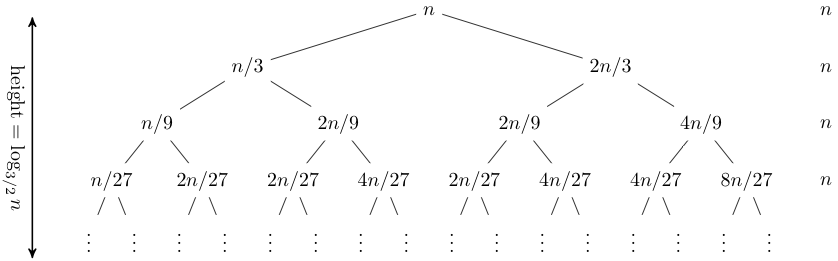
\includegraphics[width=13cm]{images/tree-1-3-2_3-1}
    \caption{Recursion tree ของการเวียนบังเกิด $T(n)=T(\frac{n}{3}) + T(\frac{2n}{3}) + n$ }
    \label{fig:tree-1-3-2-_3-1}
\end{figure}
จากรูป 4.4 จะเห็นได้ว่าทุกชั้นมีจำนวนคำสั่งรวมเท่ากันทั้งหมด คือ $n$ และความสูงของต้นไม้ คือ $log_{\frac{3}{2}} n$ (ความสูงของต้นไม้คือความยาวที่มากที่สุดจากปมรากไปยังปมใบที่มีค่าเป็น 1) จึงสรุปได้ว่า $T(n)=O(nlog_{\frac{3}{2}}n)$
\end{example}

\newpage

\subsection{Master Theorem}

Master theorem เป็นสูตรที่ใช้ในการแก้การเวียนบังเกิดในรูปแบบ
\begin{center}
$T(n)=aT(\frac{n}{b})+f(n)$
\end{center}
โดยที่ $a,b \geq 1$ และ $f(n)$ คือเวลาในการทำงานหากมีข้อมูลนำเข้า $n$ ตัว

\textbf{หมายเหตุ:} Master theorem สามารถใช้ได้ในกรณีที่ $f(n)$ มีค่าเท่ากับหรือแตกต่างจาก $n^{log_b a}$ มากๆ เท่านั้น เช่นไม่สามารถใช้แก้ $T(n)=3T(\frac{n}{3}) + nlog(n)$ ได้ เนื่องจาก $n^{log_b a}=n$ แตกต่างจาก $nlog(n)$ เพียงระดับ $log$ เท่านั้น

\begin{theorem}
ให้ $a$ และ $b$ เป็นค่าคงตัวที่ $a>0$ และ $b>1$
\begin{center}
$T(n)=aT(\frac{n}{b})+f(n)$
\end{center}
โดย $\frac{n}{b}$ หมายถึง $\lceil\frac{n}{b}\rceil$ หรือ $\lfloor \frac{n}{b} \rfloor$ อย่างใดอย่างหนึ่ง แล้ว $T(n)$ จะสามารถวิเคราะห์ได้ ดังนี้
\begin{enumerate}
\item ถ้า $n^{log_b a}<f(n)$ แล้ว $T(n)=\Theta(f(n))$
\item ถ้า $n^{log_b a}=f(n)$ แล้ว $T(n)=\Theta(f(n) \cdot log(n))$
\item ถ้า $n^{log_b a}>f(n)$ แล้ว $T(n)=\Theta(n^{log_b a})$
\end{enumerate}
\end{theorem}

\begin{example}
$T(n)=27T(\frac{n}{3}) + n^3$

ในตัวอย่าง 4.2.3 นี้ $a=27$, $b=3$, $f(n)=n^3$ จึงได้ว่า $n^{log_b a}=f(n)=n^3$ เข้ากรณีที่ 2 จึงสรุปได้ว่า $T(n)=\Theta(n^3 log(n))$
\end{example}

\begin{example}
$T(n)=2T(\frac{n}{2}) + n^2$

ในตัวอย่าง 4.2.4 นี้ $a=2$, $b=2$, $f(n)=n^2$ จึงได้ว่า $n^{log_b a}=n<f(n)=n^2$ เข้ากรณีที่ 1 จึงสรุปได้ว่า $T(n)=\Theta(n^2)$
\end{example}
